\newcommand{\psd}[1]{{\small\sffamily{\color{blue!60}#1}}}

A two dimensional test is introduced. The problem of interest is the
typical single notch square plate cracking test under tensile loading. A
unit square with a pre existing crack is clamped at the bottom
\(u_1=u_2=0\) (first boundary condition) and is loaded quasi-statically
\(u_2=u_2 + \Delta u_2\) on its top surface till the crack propagates
through its walls. So there are two Dirichlet conditions one on the top
border and one on the bottom one.

\begin{figure}[h!]
\centering
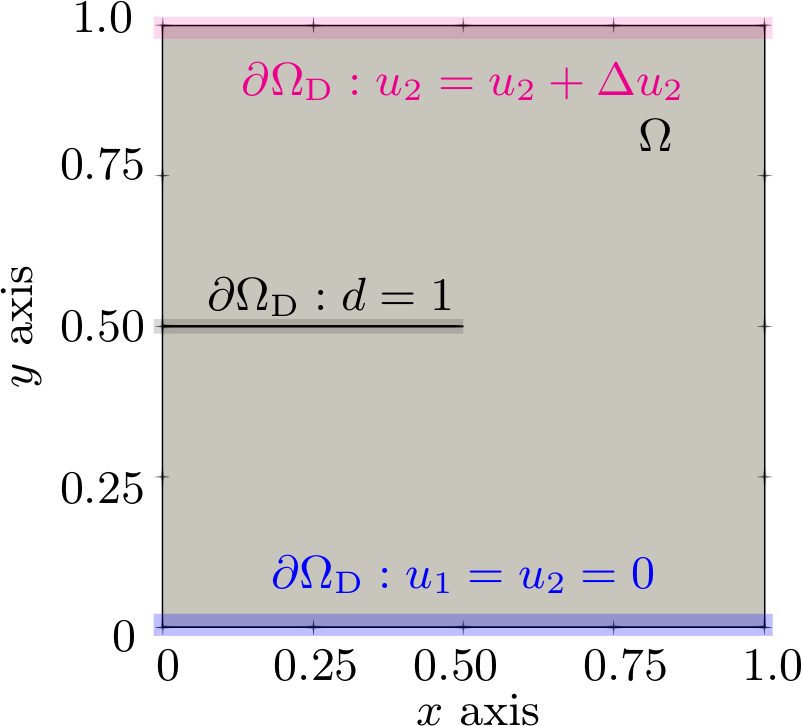
\includegraphics[width=0.3\textwidth]{./Images/square-notch.png}
\caption{Domain of the single notch square cracking problem under tensile loading. \label{bar-sd}}
\end{figure}

To model this test PSD provides hybrid phase-field modelling technique.
We use ParaView post-processing of displacement \(u\) and phase-field
\(d\) to visualise the cracking process. A PSD simulation is a two step
process, with step one being the \psd{ PSD\_PreProcess }:

\begin{lstlisting}[style=BashInputStyle]
PSD_PreProcess -dimension 2 -problem damage -model hybrid_phase_field \
-dirichletconditions 2 -postprocess ud
\end{lstlisting}

A note on flags.

\begin{itemize}
\tightlist
\item
  This is a two-dimensional problem, so we use the flag
  \psd{-dimension 2}.
\item
  This problem indeed falls under the category of damage-mechanics,
  hence the flag \psd{ -problem damage}.
\item
  We wish to solve this problem by invoking the hybrid phase-field
  problem, which is signified by the flag
  \psd{ -model hybrid\_phase\_field}.
\item
  Versed in the description above the problem contains two Dirichlet
  conditions, we signal this via the flag \psd{-dirichletconditions 2}.
\item
  Finally for this problem we use the flag \psd{-postprocess ud} which
  enables post-processing of displacement \(u\) and damage (phase-field)
  \(d\) fields.
\end{itemize}

Once the step above has been performed, we solve the problem using four
MPI processes, with the given mesh file \psd{tensile-crack.msh}. This is
step two of the PSD simulation \psd{ PSD\_Solve}.

\begin{lstlisting}[style=BashInputStyle]
PSD_Solve -np 4 Main.edp -mesh ./../Meshes/2D/tensile-crack.msh -v 0
\end{lstlisting}

\begin{figure}[h!]
\centering

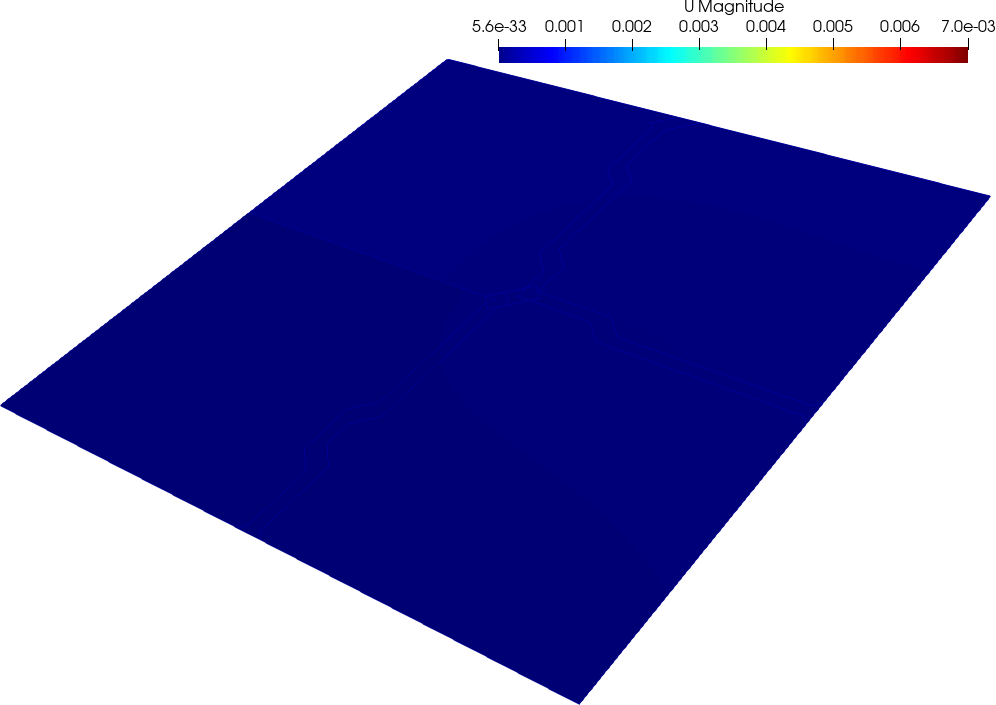
\includegraphics[width=0.24\textwidth]{./Images/u0.png}
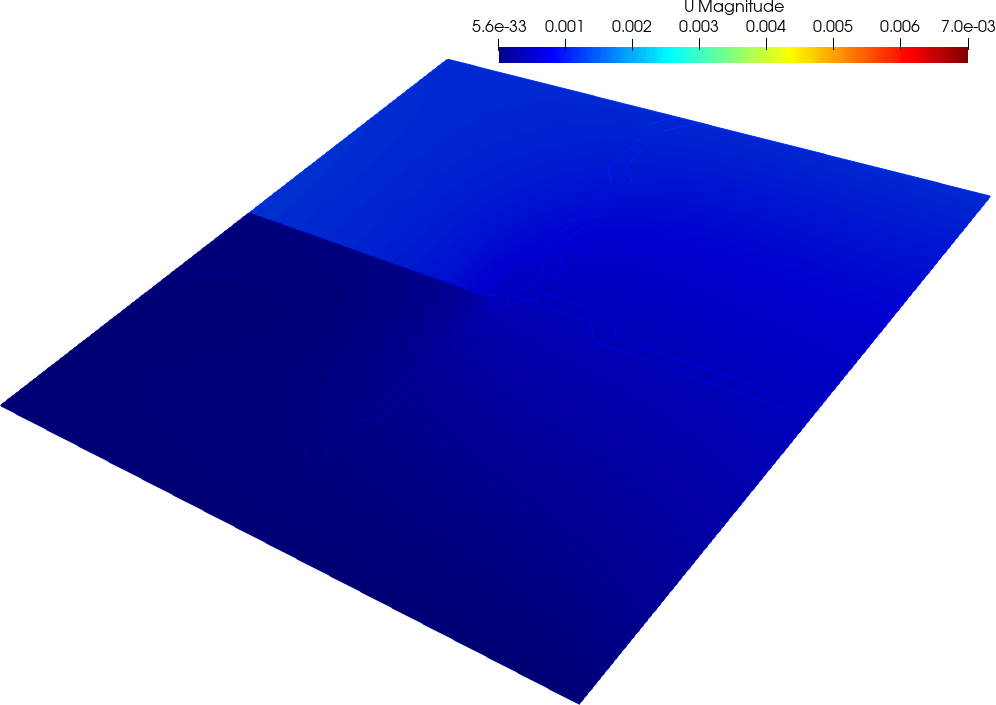
\includegraphics[width=0.24\textwidth]{./Images/u1.png}
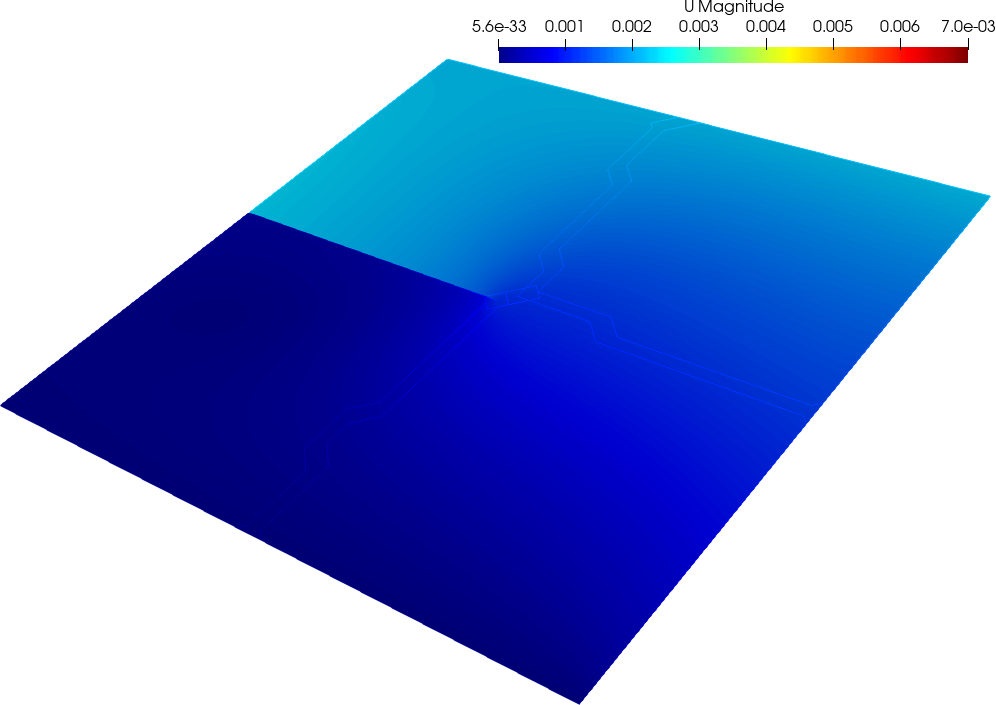
\includegraphics[width=0.24\textwidth]{./Images/u2.png}
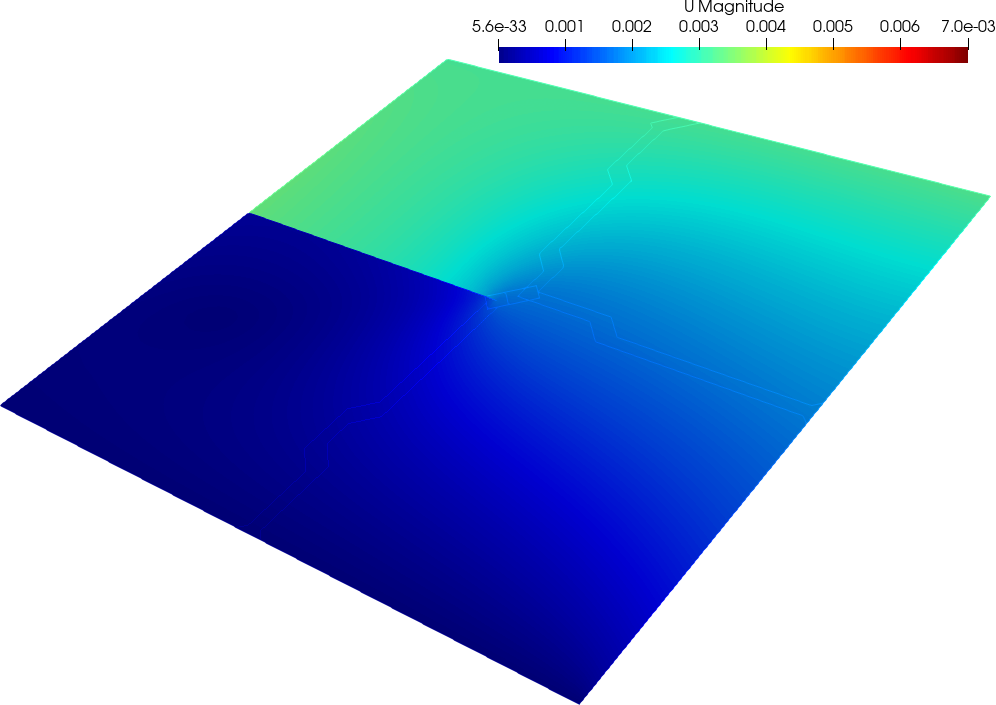
\includegraphics[width=0.24\textwidth]{./Images/u3.png}\\
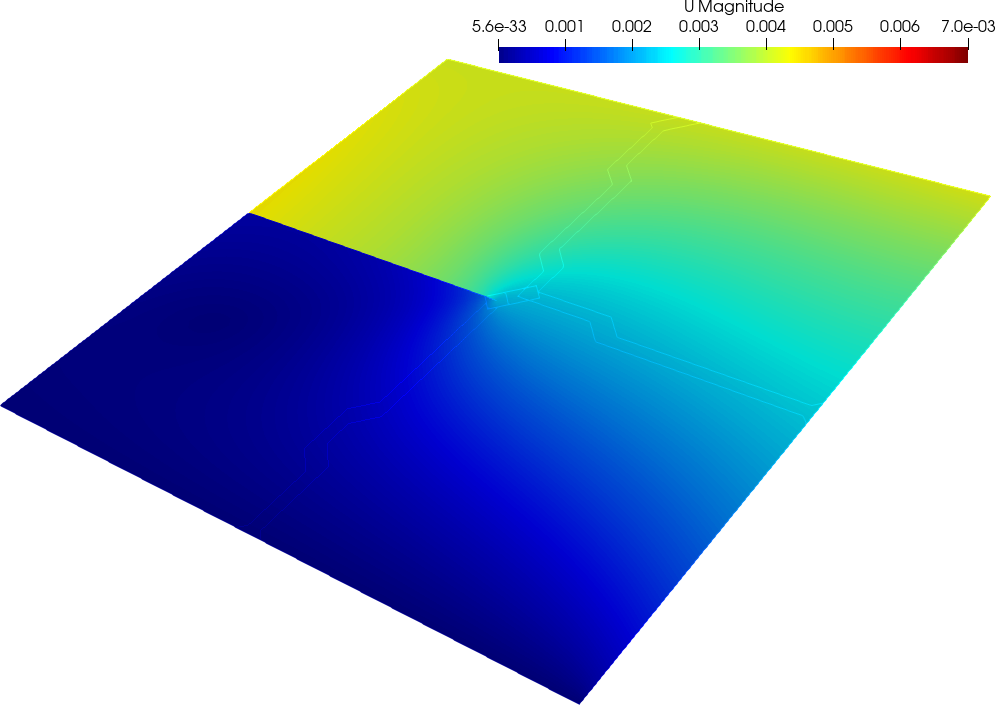
\includegraphics[width=0.24\textwidth]{./Images/u4.png}
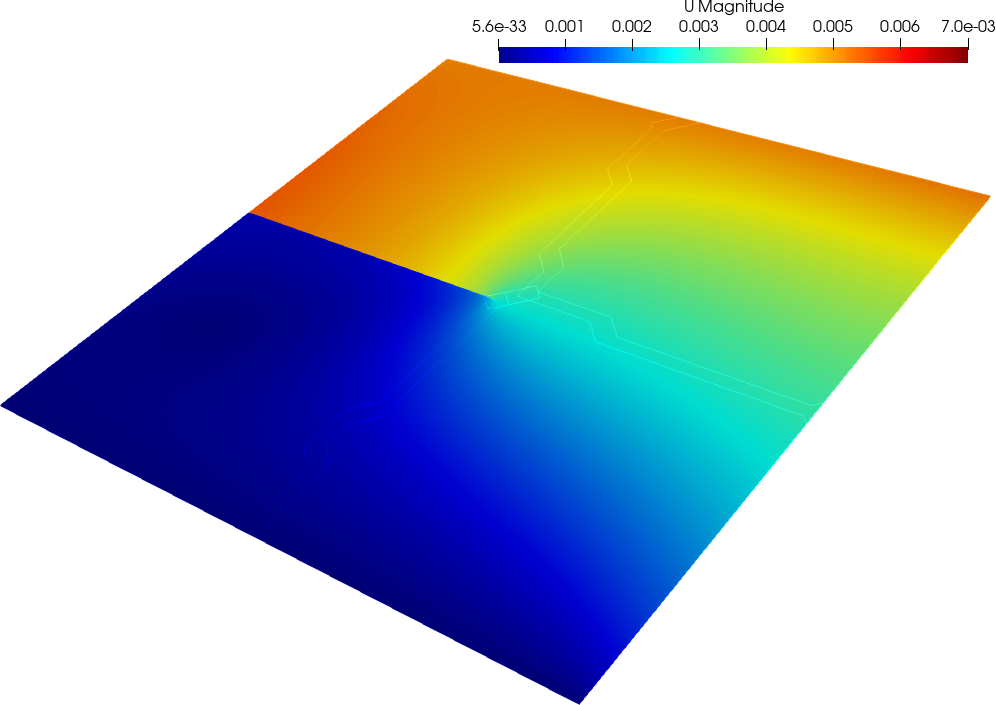
\includegraphics[width=0.24\textwidth]{./Images/u5.png}
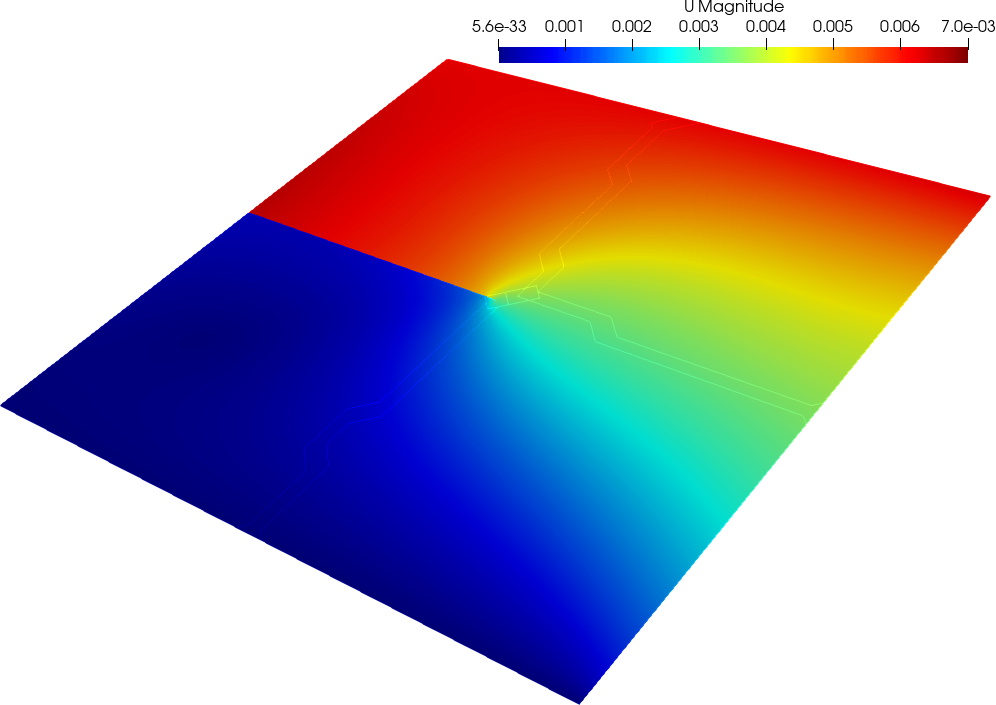
\includegraphics[width=0.24\textwidth]{./Images/u6.png}
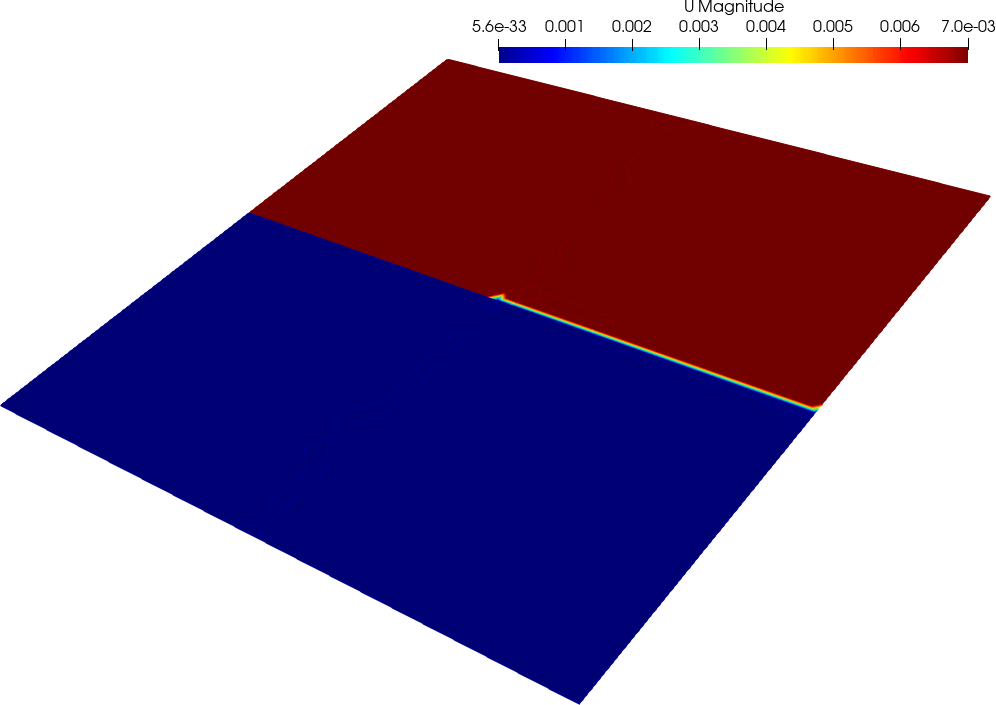
\includegraphics[width=0.24\textwidth]{./Images/u7.png}
\caption{Finite element displacement visualised for the 2D problem with ParaView at different timesteps (quasi-statics). Time progresses from left to right in a row and top to bottom when comparing rows. \label{u-fem}}
\end{figure}

\begin{figure}[h!]
\centering

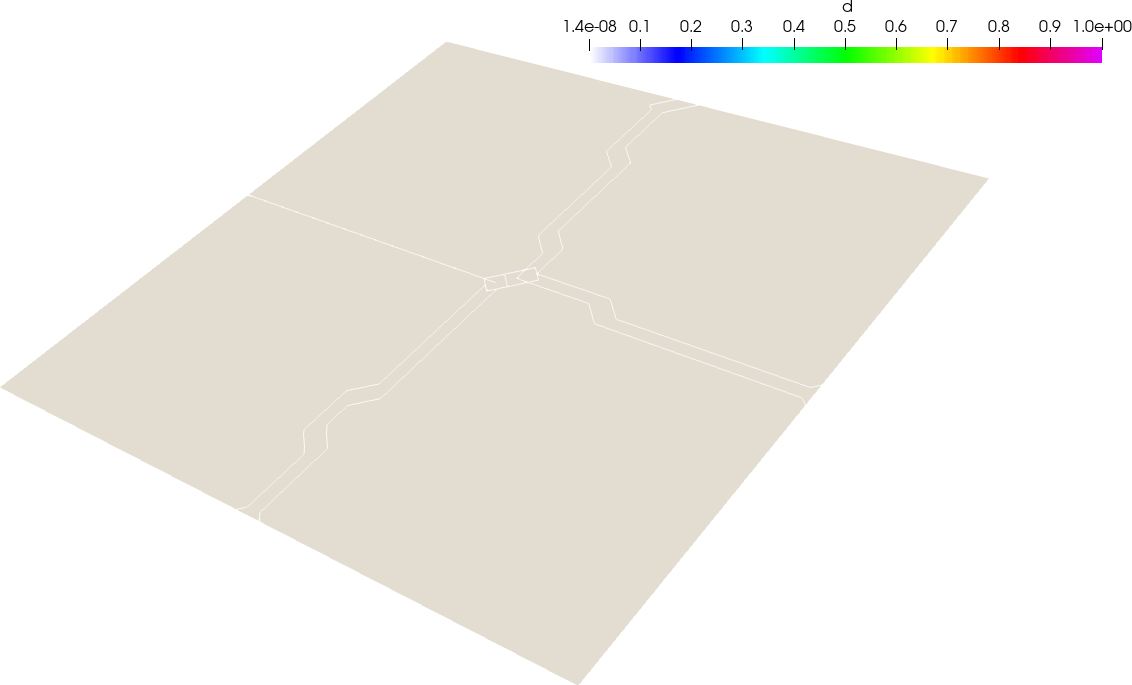
\includegraphics[width=0.24\textwidth]{./Images/d0000.png}
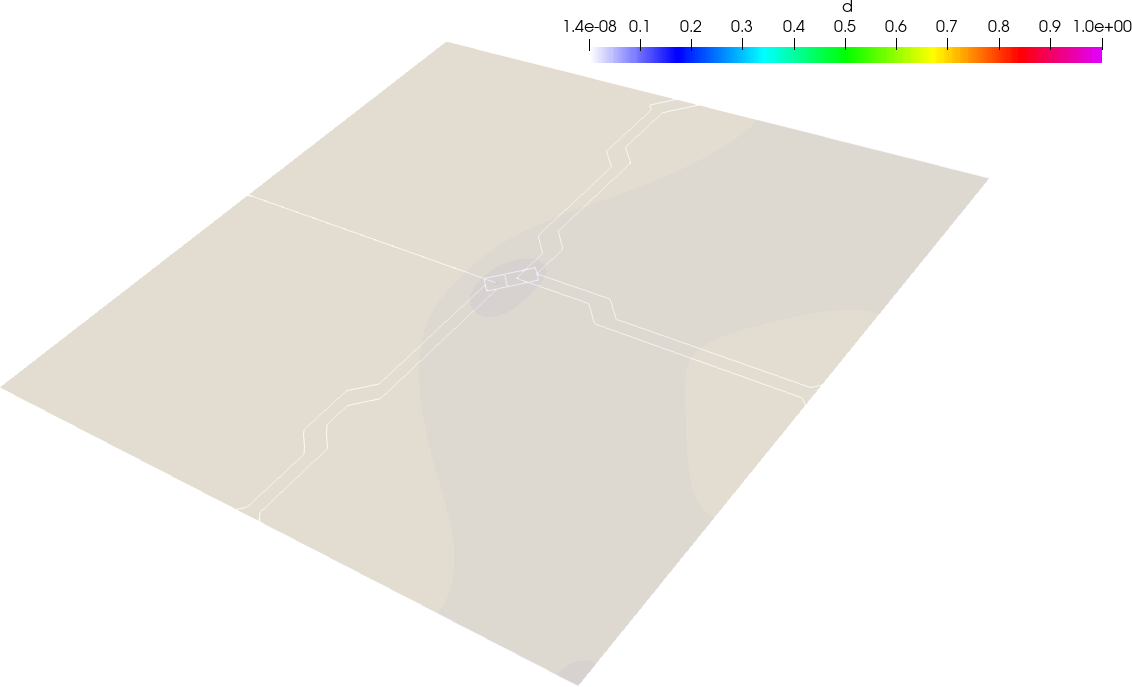
\includegraphics[width=0.24\textwidth]{./Images/d0010.png}
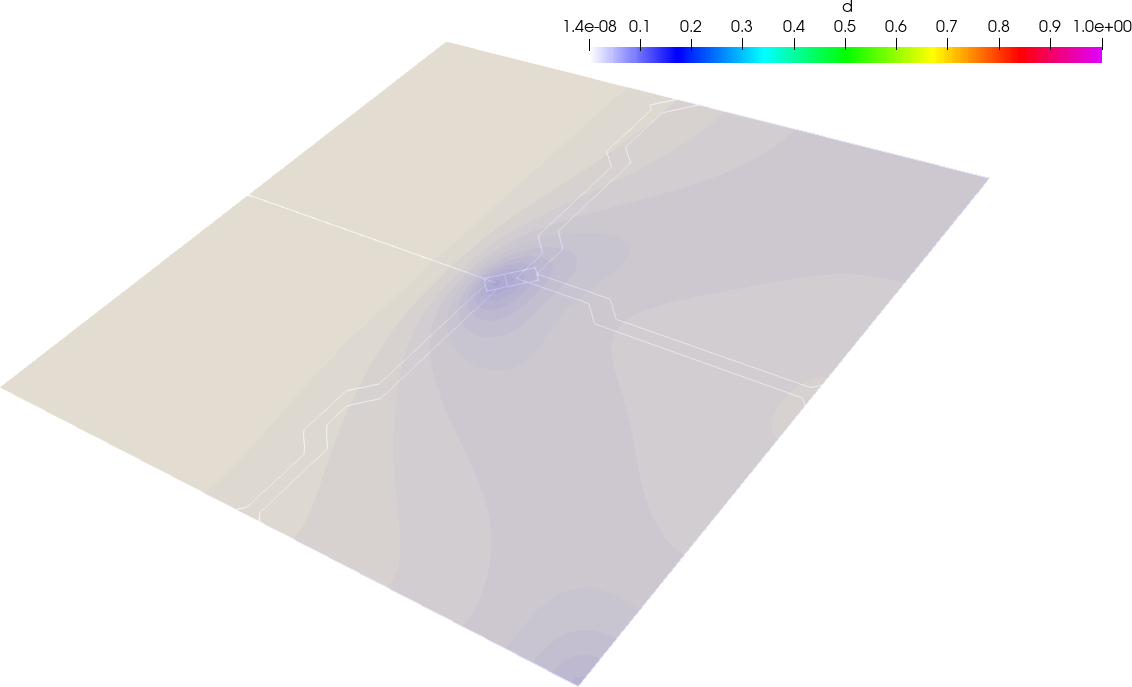
\includegraphics[width=0.24\textwidth]{./Images/d0020.png}
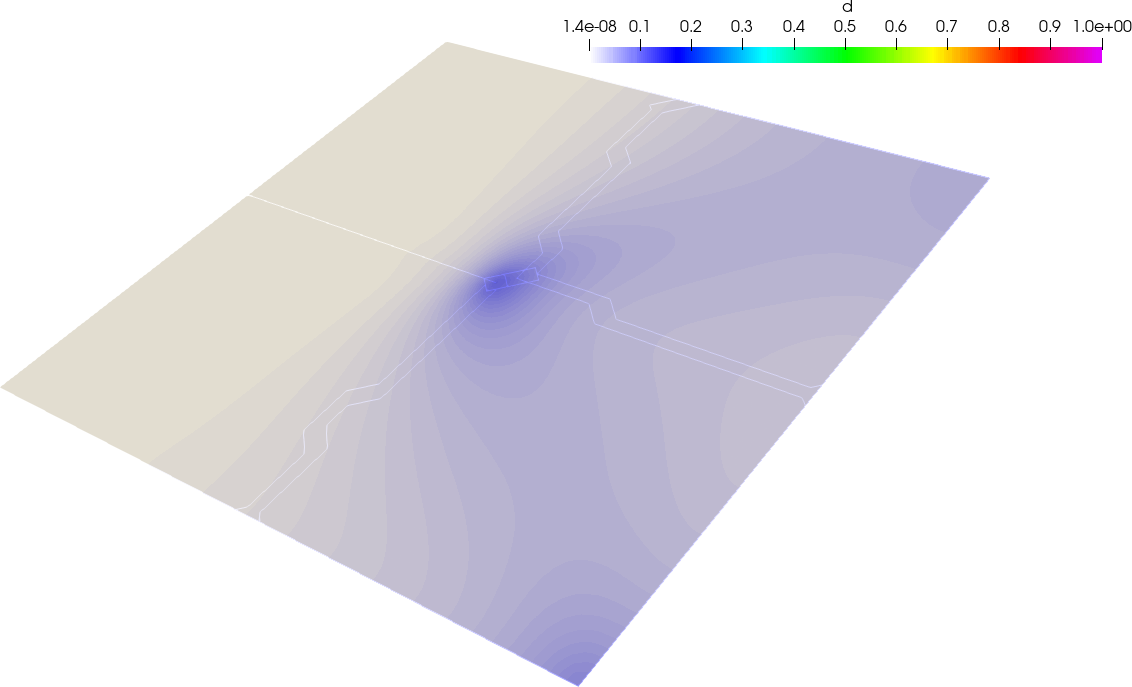
\includegraphics[width=0.24\textwidth]{./Images/d0030.png}\\
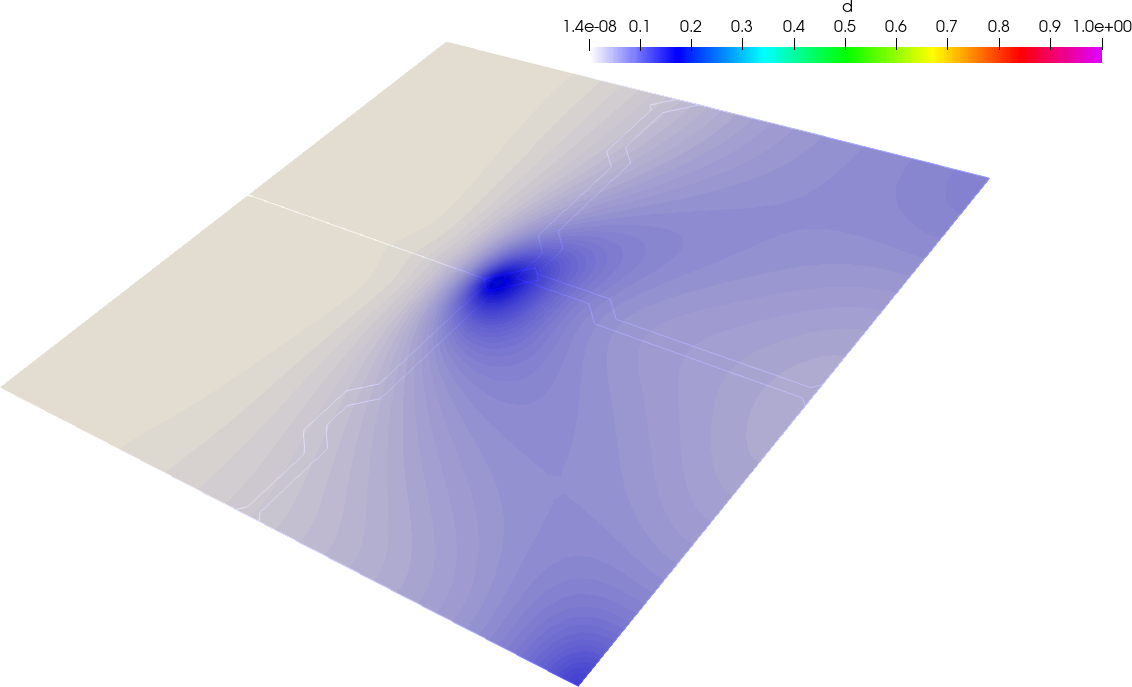
\includegraphics[width=0.24\textwidth]{./Images/d0040.png}
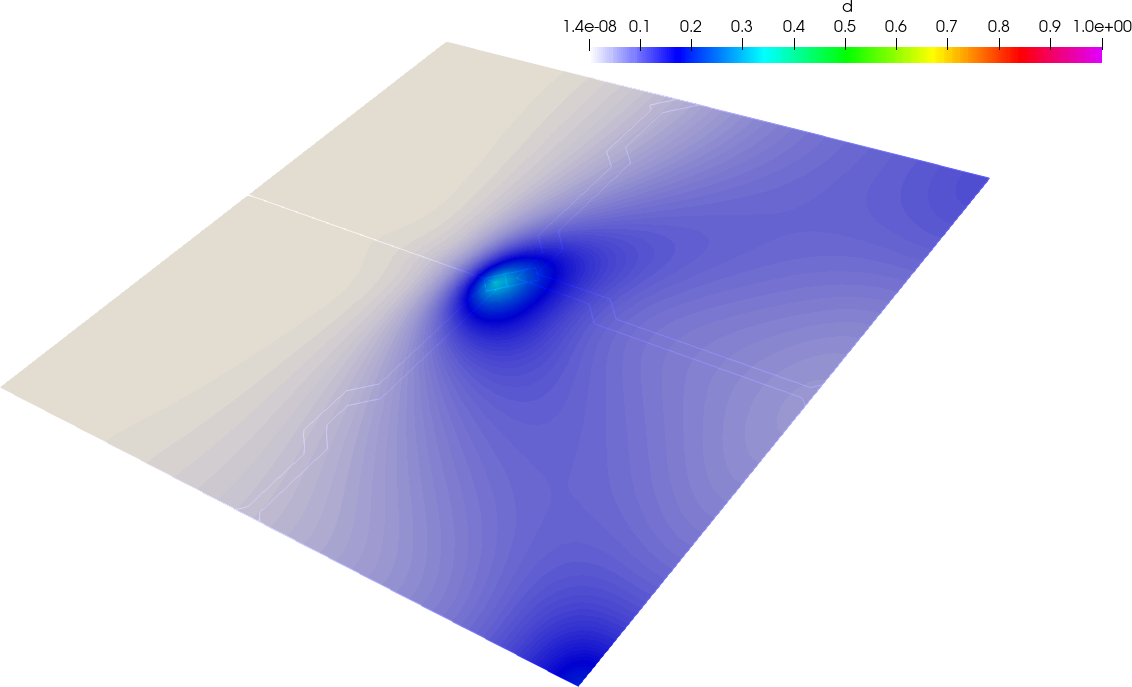
\includegraphics[width=0.24\textwidth]{./Images/d0050.png}
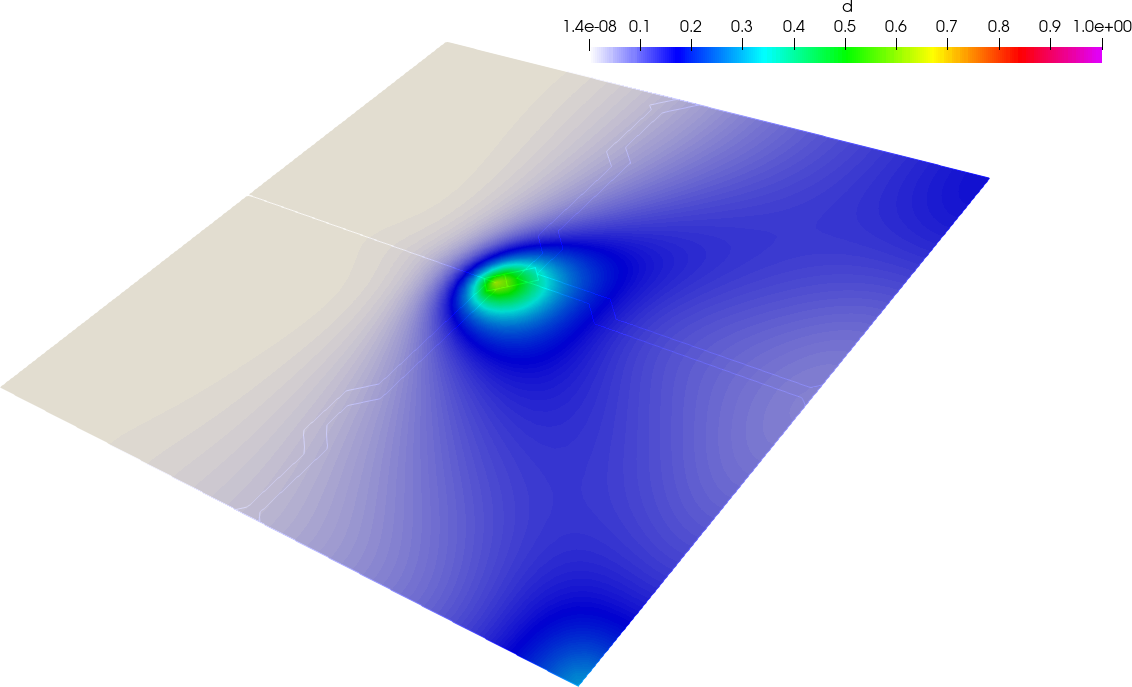
\includegraphics[width=0.24\textwidth]{./Images/d0060.png}
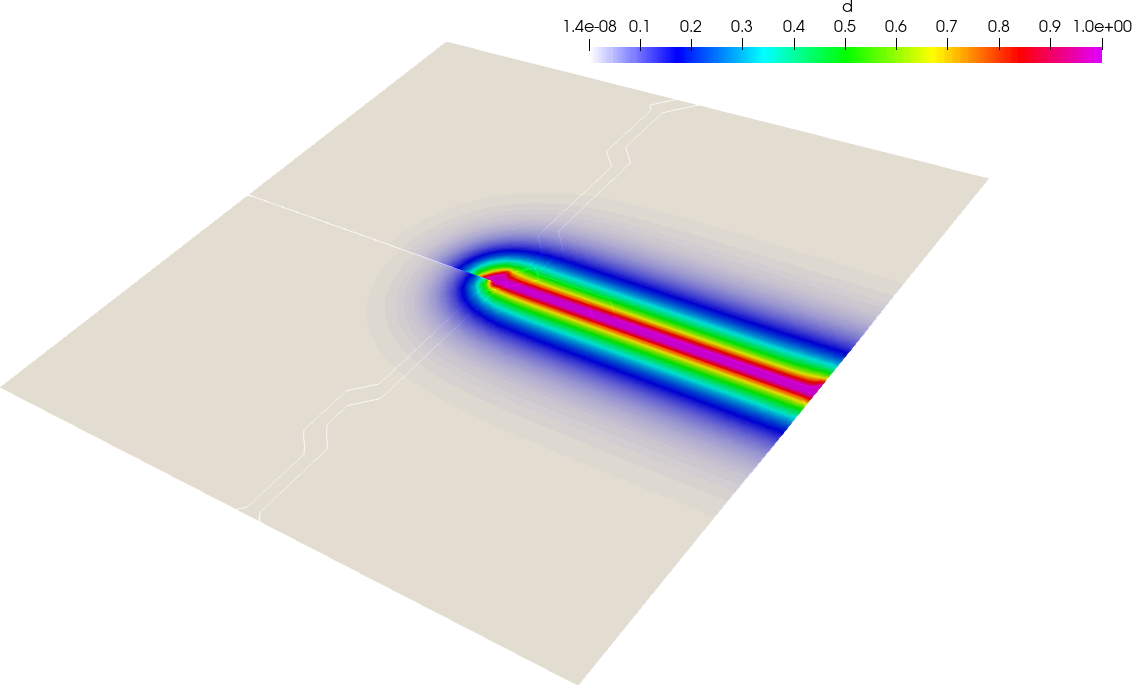
\includegraphics[width=0.24\textwidth]{./Images/d0069.png}
\caption{Finite element damage visualised for the 2D problem with ParaView at different timesteps (quasi-statics). Time progresses from left to right in a row and top to bottom when comparing rows. \label{d-fem}}
\end{figure}

Figures \ref{u-fem} and \ref{d-fem} present the finite element
displacement and damage field, which enable us to visualise the cracking
of the square plate.

\begin{figure}[h!]
\centering

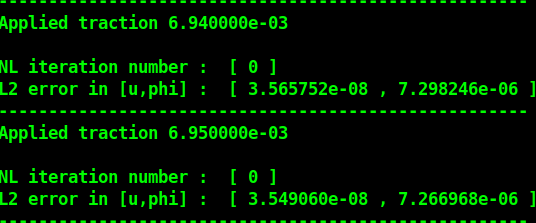
\includegraphics[width=0.6\textwidth]{./Images/terminal1.png}
\caption{Applied traction, non-linear iterations to convergence, and residual being casted onto the terminal shell. \label{term}}
\end{figure}

While this test runs, you will see on your screen the amount of traction
updated, non-linear iterations taken to converge per-quasi-time-step and
residue of \(u\) and \(d\). See figure \ref{term} that shows the
screenshot of the terminal while the test was running. In order to
construct your own test case try editing the \psd{ControlParameters.edp}
file.
